\documentclass[11pt,letter]{article}
\usepackage[utf8]{inputenc}
\usepackage{amsmath}
\usepackage{amsfonts}
\usepackage{amssymb}
\usepackage{enumitem}
\usepackage[margin=1in]{geometry}
\usepackage{graphicx}
\usepackage{verbatim}
\setlist[enumerate]{itemsep=0mm}
\setlength\parindent{0pt}
\renewcommand{\thesubsection}{\thesection.\alph{subsection}}


\author{Haosu Tang}
\title{Project C}

\begin{document}

\maketitle

\section{Beta}
I chose BA (Boeing company) to do this analysis. Data range: 2008-01-01 to 2009-12-31, during which the financial crisis happened and the market was highly volatile.\\

\textbf{(a)}. Time series plots of the 3-month rolling beta, S\&P 500 and scatter plot of beta vs S\&P500.
\begin{center}
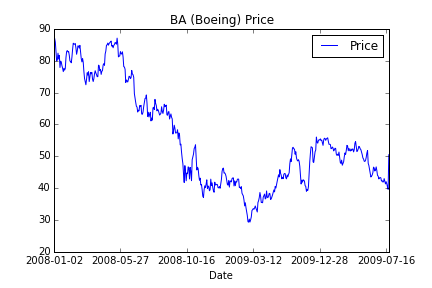
\includegraphics[width=4in,keepaspectratio]{1aBA}
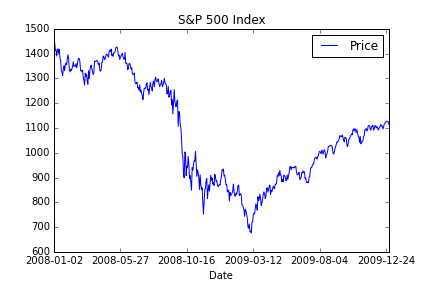
\includegraphics[width=4in,keepaspectratio]{1aSP}
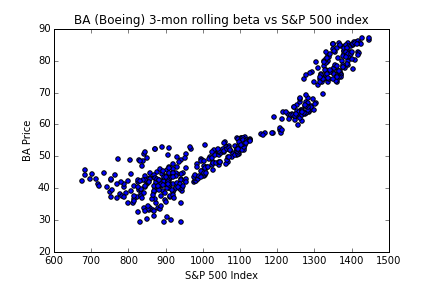
\includegraphics[width=4in,keepaspectratio]{1aBASPscatter}
\end{center}


\textbf{(b)}. A scatter plot of 1-day stock returns vs. the SPTR 1-day return and linear regression line.
\begin{center}
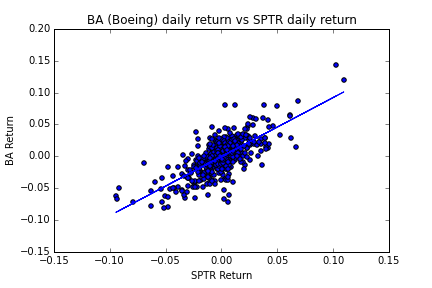
\includegraphics[width=4in,keepaspectratio]{1bBARetSPTRscatter}
\end{center}
Equation for linear regression:
\begin{itemize}
\item (With intercept): $ \hat{y} = -0.00041234 + 0.92471118 \hat{x}$
\item (Intercept = 0): $ \hat{y} = 0.92509641 \hat{x}$
\end{itemize}


\textbf{(c)}. A scatter plot of 1-day stock returns vs. the VIX 1-day return and the linear regression line.
\begin{center}
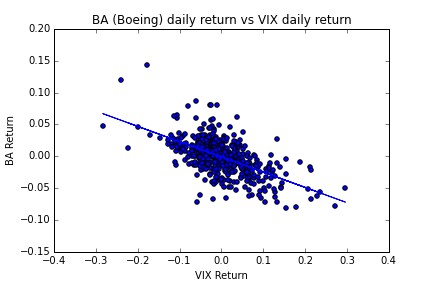
\includegraphics[width=4in,keepaspectratio]{1cBARetVIXscatter}
\end{center}
\begin{itemize}
\item (With intercept): $ \hat{y} = -0.00084599 -0.23941314 \hat{x}$
\item (Intercept = 0): $ \hat{y} = -0.23939968 \hat{x}$
\end{itemize}


\section{Performance attribution}

\textbf{(a)}. Using data from strategy "Contra01" from OLAP database for 2005-2009, analyze the performance. I plotted the "Weighted Return Tc" and "1 month Volatility" for this period. To note, "1 month Volatility" and "3 month Volatility" have exactly the same values. Given these large volatility measures, I think the these values are already annualized. Otherwise, volatility should multiply by square root of number of the months and Sharpe ratio divide. With risk free rate 0, I make table for the annualized return, volatility and Sharpe ratio.\\

Case 1: \textit{Overall}
\begin{center}
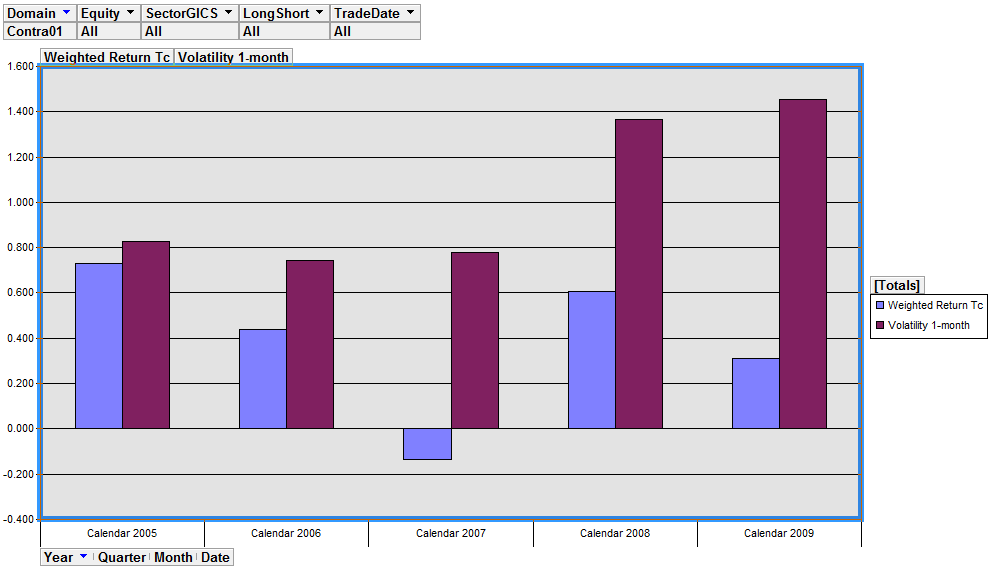
\includegraphics[scale=0.5,keepaspectratio]{2a_overall}
\newline

\begin{tabular}{l | l l l}
Year & Return & Volatility & Sharpe Ratio\\
\hline
2005	 & 73.18\% & 82.85\% & 0.8833\\
2006	 & 43.86\% & 74.49\% & 0.5888\\
2007	&-13.61\%	&77.76\%	&-0.1750\\
2008	&60.68\%	&136.51\%	&0.4445\\
2009	&31.09\%	&145.30\%	&0.2140\\
\hline
Total&	195.20\%	&100.36\%	&1.9450
\end{tabular}
\end{center}


Case 2: \textit{Long}
\begin{center}
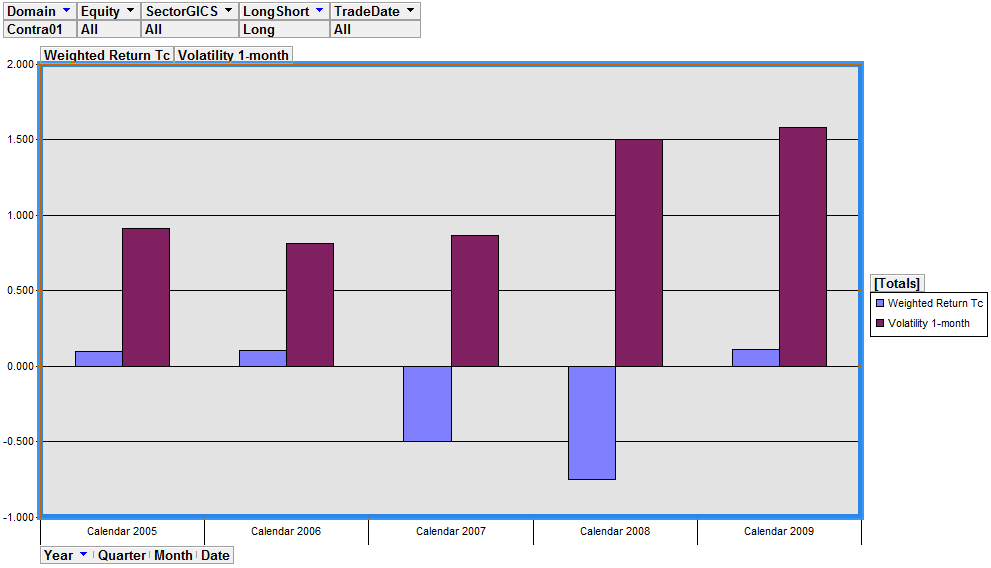
\includegraphics[scale=0.5,keepaspectratio]{2a_long}
\newline

\begin{tabular}{l|lll}
Year & Return & Volatility & Sharpe Ratio\\
\hline
2005	&10.02\%	&91.67\%	&0.1093\\
2006	&10.70\%	&81.66\%	&0.1310\\
2007	&-49.36\%	&86.45\%	&-0.5710\\
2008	&-74.63\%	&150.30\%	&-0.4965\\
2009	&11.09\%	&158.36\%	&0.0700\\
\hline
Total&	-92.18\%	&110.41\%	&-0.8349
\end{tabular}
\end{center}


Case 3: \textit{Short}
\begin{center}
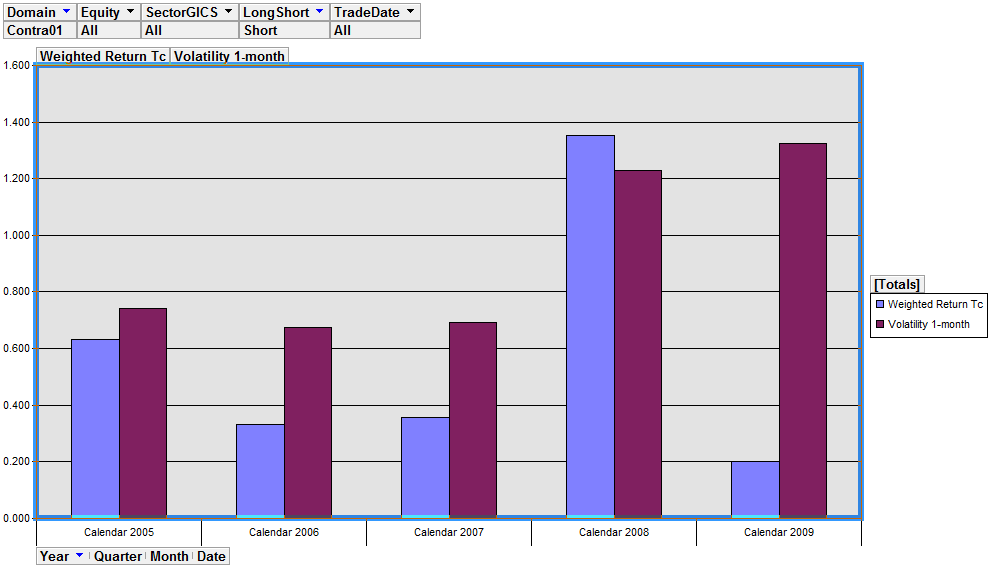
\includegraphics[scale=0.5,keepaspectratio]{2a_short}
\newline

\begin{tabular}{l|lll}
Year & Return & Volatility & Sharpe Ratio\\
\hline
2005	&63.16\%	&74.07\%	&0.8527\\
2006	&33.15\%	&67.33\%	&0.4924\\
2007	&35.75\%	&69.09\%	&0.5174\\
2008	&135.31\%	&122.76\%	&1.1022\\
2009	&20.00\%	&132.30\%	&0.1512\\
Total&	287.38\%	&90.34\%	&3.1811
\end{tabular}
\end{center}


\textbf{(b)}. Regrouping the data by SIC sector and filter only the 2006. Manufacturing contributes the most to the absolute overall return. It contributes 801.83\% to the overall 1617.46\%, i.e. 49.57\%.\\

Plot and table:
\begin{center}
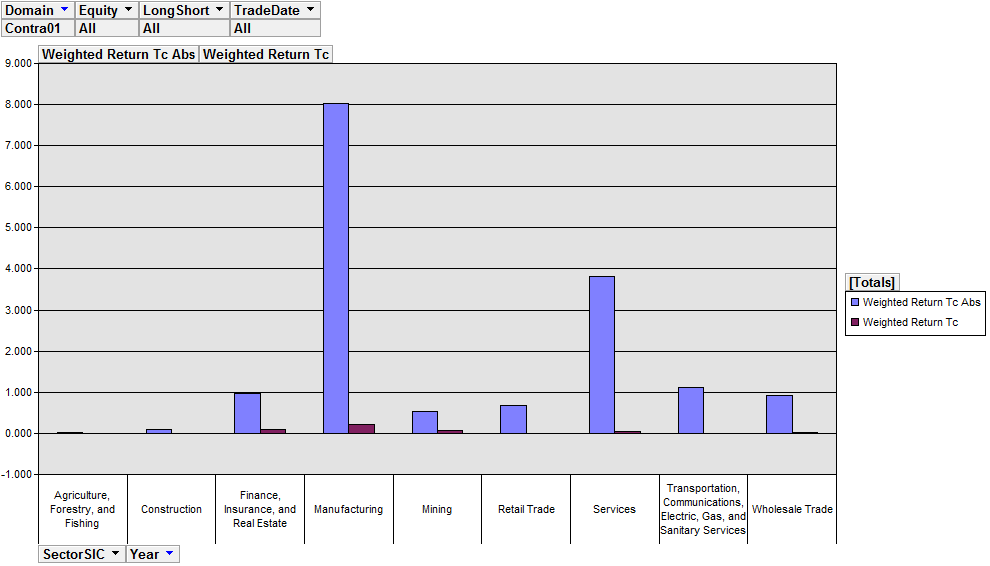
\includegraphics[scale=0.5,keepaspectratio]{2b}
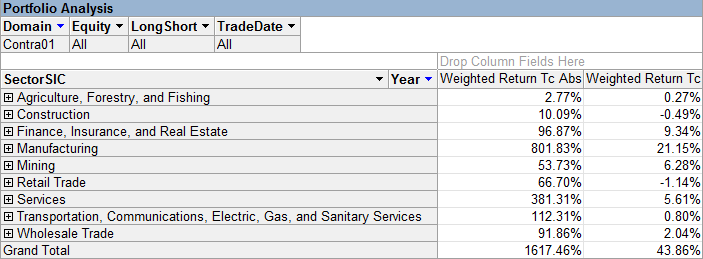
\includegraphics[scale=0.5,keepaspectratio]{2b_2}
\end{center}

\textbf{(c)}. Regrouping the data by GICS sector and filter only the 2006. Information technology contributes the most to the absolute overall return. It contributes 266.69\% to the overall 895.52\%, i.e. 29.78\%.\\

Plot and table:
\begin{center}
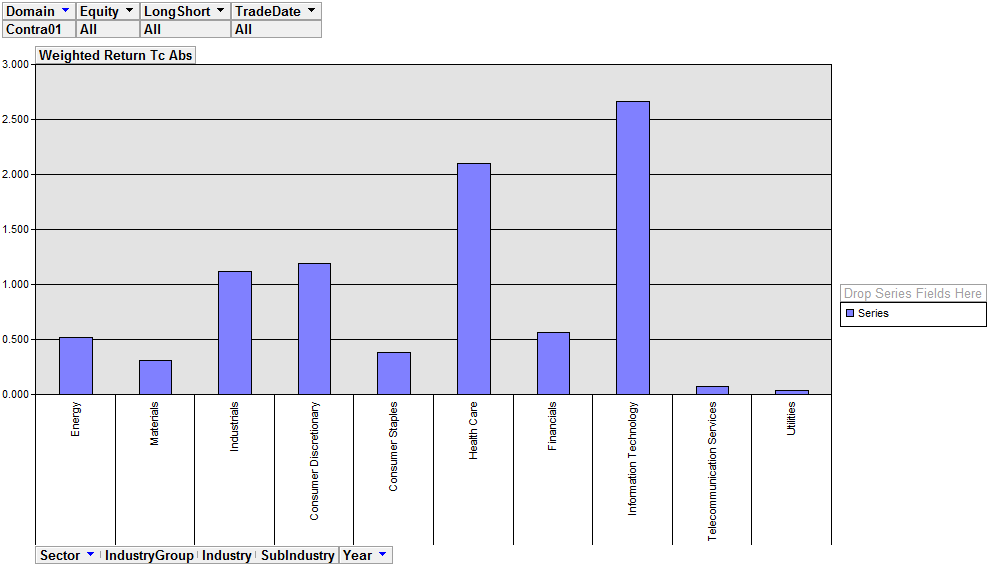
\includegraphics[scale=0.5,keepaspectratio]{2c}
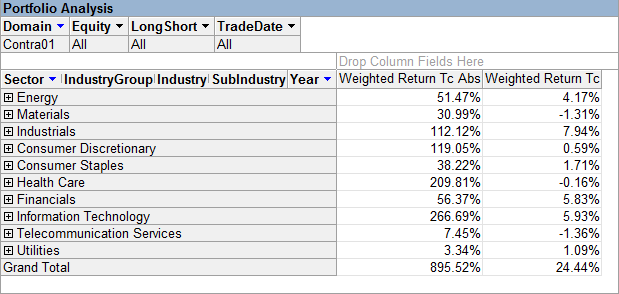
\includegraphics[scale=0.5,keepaspectratio]{2c_2}
\end{center}

\textbf{(d)}. The time series plot of strategy one-day return and plot reorganized into ascending order:

\begin{center}
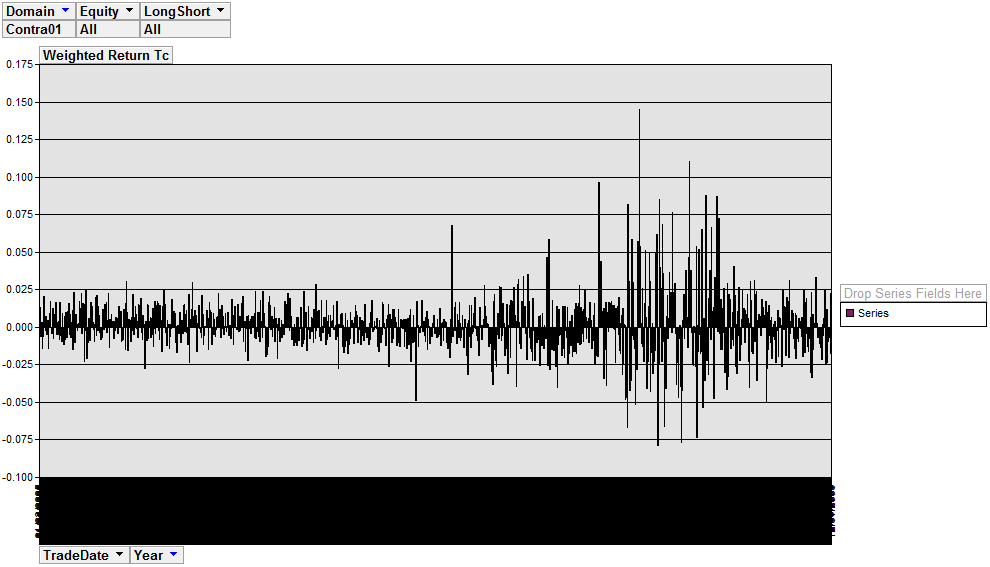
\includegraphics[scale=0.5,keepaspectratio]{2d}
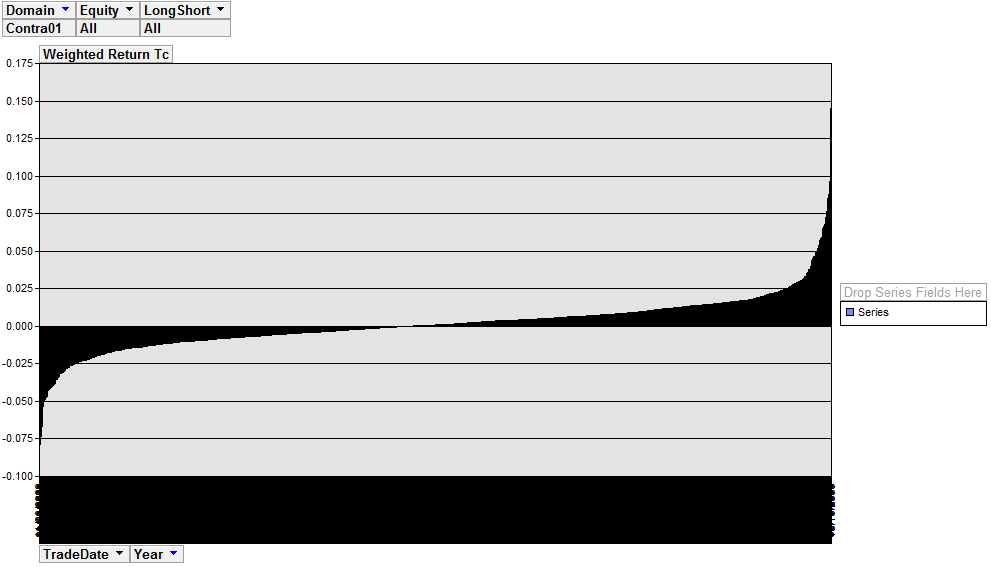
\includegraphics[scale=0.5,keepaspectratio]{2d_2}
\end{center}

This returns 1260 observations. The last one is total, so altogether 1259 observations in this 5-year range. 673 of them are positive (>0), 6 returns are 0, and 580 are negative, corresponding 53.46\% winners and 46.07 \% losers. Of all the winners, median return is 0.85\%. Of all the losers, median return is -0.82\%.

\section{Risk measurement}

\textbf{(a)}. I extracted daily weight data for each sector over the period 2005-2009 in the pivot table. The following shows a table of max (highest), min (lowest) and mean of the 1259 days.

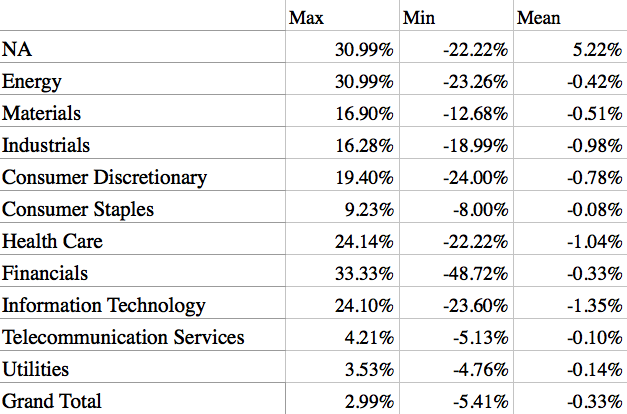
\includegraphics[scale=0.4,keepaspectratio]{3a}

Among these sectors, \textit{Comsumer Staples, Telecommunication Services, Utilities} are ones stayed within $\pm 10\%$ of the portfolio weight throughout.\\

\textbf{(b)}.On 9/15/12008, the GICS sector weights are: 
NA	11.27\%; Energy	-7.04\%; Materials	0.00\%; Industrials	-2.82\%; Consumer Discretionary	-8.45\% Consumer Staples	-1.41\%; Health Care	7.04\%; Financials	-2.82\%; Information Technology	5.63\%; Grand Total	1.41\%.


The most unbalanced position is NA 11.27\%, which are investments cannot be categorized in the sectors. The long positions sum up to be 23.94\%. Total short is 22.54\%. The portfolio return on that day is -8.06\%.\\

\textbf{(c)}. On 2/27/2007, the GICS sector weights are:
NA	6.10\%; Energy	-1.22\%; Materials	0.00\%; Industrials	4.88\%; Consumer Discretionary	1.22\%; Consumer Staples	2.44\%; Health Care	0.00\%; Financials	1.22\%; Information Technology	-14.63\%; Telecommunication Services	1.22\%; Grand Total	1.22\%.


The most unbalanced position is Information Technology -14.63\%. The long positions sum up to be 17.08\%. Total short is 15.85\%. The portfolio return on that day is -4.41\%.\\


\textbf{(d)}. Such strategy will not be market neutral on its own. Unlike the original strategy of looking at all universe of the securities tradable and developing weights that can be made market-neutral, the sub-strategy will be correlated with other sectors and will not be market neutral standing on its own. As Prof. Mende pointed out in the forum: The signals depend only on the individual stock returns relative to the market without any other references or inputs. Therefore there is no reason to expect a priori that the sectors would be neutral.

Plots of the \textit{net} long/short exposure:

\begin{center}
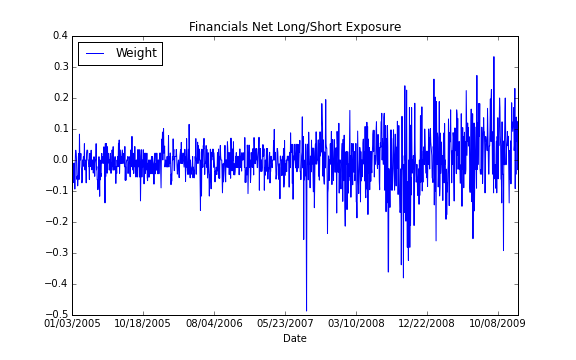
\includegraphics[width=4in,keepaspectratio]{3d}
\end{center}

Plots of the \textit{gross} long/short exposure, where blue stands for the long positions, and green short:

\begin{center}
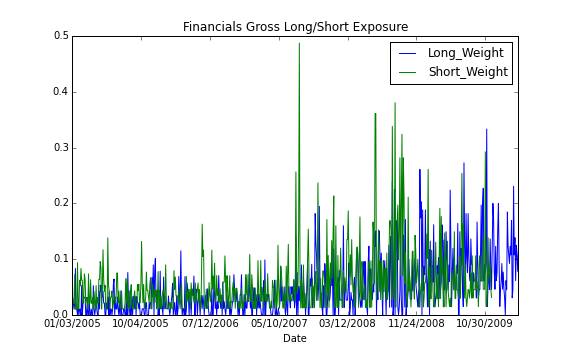
\includegraphics[width=4in,keepaspectratio]{3d_2}
\end{center}

The substrategy became more volatile (larger variance) throughout this time frame, due to the highly volatile market.

\section{Correlation dynamics}





%
%
%
%(a). Plot and label a bar graph with the time series of daily portfolio returns and one with the time series of daily market returns.
%
%I used Access to get equity universe data from obelix.mit.edu and query it to form a table consisting of:
%\begin{enumerate}
%\item date d, an integer number starting from 7543 to 10570, representing trading dates between 1/1/1990 and 12/31/2001,
%\item stock id, if the flag is 1,
%\item log return r.
%\end{enumerate}
%
%And using Matlab, for each day, 
%\begin{enumerate}
%\item transform the log return to real return,
%\item calculate mean return and each stock's absolute return,
%\item assgin normalized weight to each stock,
%\item calculate the portfolio return through dot product $pi_t= w_{t-1}^TR_t$.
%\end{enumerate}
%(The code is attached at the end of this write-up.)
%
%The time series plot for the return of the mean reversion portfolio:
%
%\begin{center}
%\includegraphics[width=4in,keepaspectratio]{Mean_rev}
%\end{center}
%
%And comparing to the time series plot for the return of the market:
%
%\begin{center}
%\includegraphics[width=4in,keepaspectratio]{Market}
%\end{center}
%
%(b). The mean annualized return, volatility, and Sharpe ratio of the strategy and of the market average. The annualized return I calculated using compounded return and then annualize: $\sqrt[n]{\Pi(1+r_i)}-1$. Volatility is simply overall daily standard deviation multiplied by $\sqrt{252}$ (252 trading days). And Sharpe ratio is calculated by dividing the annualized return by volatility, assuming risk free rate 0.
%\begin{verbatim}
%strat_Annu_r = 22.164171668343567
%
%strat_Annu_vol = 0.213763539224245
%
%strat_Annu_SR = 1.036854636145064e+02
%
%market_Annu_r = 0.169325792411088
%
%market_Annu_vol = 0.092115857155619
%
%market_Annu_SR = 1.838182888805254
%\end{verbatim}
%
%(c). Consistency and stationarity: Time series consistency and stationarity is defined as preserving a constant mean throughout time and having a time-independent well defined autocovariance. Judging from the the two time series plots, there is not serial correlation and clustering effect, and for both cases the means and covariances are more or less constant. However, the market variances do seem a bit inflated between 2000-3000 (about 1997-2001), suggesting a more volatile market. Therefore, the consistency and stationarity can be assumed valid in this case for ease of analysis, but the increase in variance one should bear in mind.
%
%\begin{center}
%\includegraphics[width=4in,keepaspectratio]{Mean_rev_refline}
%\end{center}
%
%(d). I define unusual outlier dates as those larger than $\bar{R} \pm 4S$, where $S$ is the standard deviation. Under the assumption of returns being normally distributed, a 4 standard deviation away is less than 0.001\% likely. The results are:
%\begin{verbatim}
%[7713, 7863, 8032, 8457, 8458, 9174, 9484, 9817, 9840, 10092, 10448, 10486]
%\end{verbatim}
%
%These correspond to these dates:
%09/04/1990, 04/09/1991, 12/06/1991, 08/12/1993, 08/13/1993, 06/13/1996, 09/04/1997, 12/30/1998, 02/03/1999, 02/02/2000, 07/02/2001, 08/24/2001.\\
%
%And I defined the outlier stocks as the assigned weight of more than 10\%, which means for the previous day, this stock behaves abnormally (either extremely high return or extremely low return) against the market average. These stocks and the corresponding weights are:
%\begin{verbatim}
%   63511: 0.113350040847314
%   30761: 0.147599964114200
%   55336: 0.119772746634528
%   48389: 0.100088821163926
%   61524: 0.108428751055292
%   66545: 0.107852786103411
%   34841: 0.135585573246371
%\end{verbatim}
%
%These outlier dates and stocks will have an effect on overall stock returns as it scales the return of the total portfolio and gets magnified throughout the time series.
%
%(e) The correlation between the strategy and the market:
%\begin{verbatim}
%corr(strategy, market) = 0.069865960126031
%\end{verbatim}
%To test whether or not the strategy is market-neutral, I ran a counter-example: I revert all the market returns to their negative and keep the strategy unchanged. In this case, the market is downward trending in the time frame, however, the strategy is able to yield the same return after all.
%\begin{verbatim}
%strat_Annu_r2 = 22.164171668343528
%
%market_Annu_r2 = -0.152124918872277
%
%corr(strategy, market2) = -0.069865960126031
%\end{verbatim}
%As can be seen from this circumstance, the market return is now negative, but the strategy return remains positive unchanged. Essentially, the "Mean reversion strategy" after all is related to the trend in the market and bet it to be reverting and is thus unchanged in this case. And the correlation is now negative. This suggests the strategy is also market neutral.\\
%
%(f) The correlation between long and short positions. It is calculated by recording long positions and short positions individually and finding the correlation:
%\begin{verbatim}
%corr(long, short) = -0.261439839425657
%\end{verbatim}
%
%(g) This simulation is purely imaginary and cannot be realistic due to a number of reasons. Some are:
%\begin{enumerate}
%\item \textbf{Trading cost.} To rebalance a daily portfolio of 690 stocks induces extremely high trading costs. The high return will definitely not sustain under this condition.
%
%\item \textbf{Slippage.} In this simulation I used daily return, while in real time it would not be the case. It is very hard to bet on the price one wants and slippage may occur due to multiple reasons (timing, unfilled orders etc).
%
%\end{enumerate}
%
%Counting various factors, my guess of the annualized return should be much lower than the market return - this strategy cannot beat the market. It is hard to find a actual number. The idea is the daily return of the simulation is approximately 1.2\%, but then the trading cost of 690 stocks would account for approximately $690*2*0.01\%$ assuming 0.01 transaction cost. This yields high negative return! The data issues need to be considered related to the strategy is incompleteness of data, possible wrongly recorded data, null/NaN data, and requirement for finer data.
%
%\section{A family of strategies.}
%
%$k$ from 1 to 10:\\
%
%\begin{tabular}{l | l l l}
%k & Return & Volatility & Sharpe Ratio\\
%\hline
%1 & 22.16 & 0.2138 & 103.69 \\
%2 & 0.3593 & 0.1493 & 2.407\\
%3 & 0.2019 & 0.1441 & 1.401\\
%4 & 0.1382 & 0.1332 & 1.037\\
%5 & 0.04871 & 0.1354 & 0.3596\\
%6 & 0.1642 & 0.1363 & 1.2051\\
%7 & 0.01336 & 0.1280 & 0.1044\\
%8 & 0.09610 & 0.1293 & 0.7430\\
%9 & 0.01090 & 0.1266 & 0.08611\\
%10 & 0.00009533 & 0.1292 & 0.0007377\\
%\end{tabular}
%\newline
%\newline
%There is a significant decreasing trend in return, which suggests mean reversion feature dies out with time.\\
%
%Uploaded to Obelix. Access sql query is extremely painful - took more than 6 hours to map t to d.\\
%
%Check results:\\
%1. Row numbers of ID 919122398:\\
%\includegraphics{check1}\\
%2. Check 10 rows:\\
%\includegraphics{check2}
%
%\includegraphics[width=4in,keepaspectratio]{check1}

\end{document}